% !TeX program = pdflatex
% !BIB program = bibtex
% Template LaTeX file for DAFx-19 papers

%------------------------------------------------------------------------------------------
%  !  !  !  !  !  !  !  !  !  !  !  ! user defined variables  !  !  !  !  !  !  !  !  !  !  !  !  !  !
% Please use these commands to define title and author(s) of the paper:
\def\papertitle{On Bad Circuit Modelling}
\def\paperauthorA{Jatin Chowdhury}

% Authors' affiliations have to be set below

%------------------------------------------------------------------------------------------
\documentclass[twoside,a4paper]{article}
\usepackage{dafx_19}
\usepackage{amsmath,amssymb,amsfonts,amsthm}
\usepackage{euscript}
\usepackage[latin1]{inputenc}
\usepackage[T1]{fontenc}
\usepackage{ifpdf}

\usepackage[english]{babel}
\usepackage{caption}
\usepackage{subfig} % or can use subcaption package
\usepackage{xcolor}

\setcounter{page}{1}
\ninept

\usepackage{times}
% Saves a lot of ouptut space in PDF... after conversion with the distiller
% Delete if you cannot get PS fonts working on your system.

% pdf-tex settings: detect automatically if run by latex or pdflatex
\newif\ifpdf
\ifx\pdfoutput\relax
\else
   \ifcase\pdfoutput
      \pdffalse
   \else
      \pdftrue
\fi

\ifpdf % compiling with pdflatex
  \usepackage[pdftex,
    pdftitle={\papertitle},
    pdfauthor={\paperauthorA},
    colorlinks=false, % links are activated as colror boxes instead of color text
    bookmarksnumbered, % use section numbers with bookmarks
    pdfstartview=XYZ % start with zoom=100% instead of full screen; especially useful if working with a big screen :-)
  ]{hyperref}
  \pdfcompresslevel=9
  \usepackage[pdftex]{graphicx}
  \usepackage[figure,table]{hypcap}
\else % compiling with latex
  \usepackage[dvips]{epsfig,graphicx}
  \usepackage[dvips,
    colorlinks=false, % no color links
    bookmarksnumbered, % use section numbers with bookmarks
    pdfstartview=XYZ % start with zoom=100% instead of full screen
  ]{hyperref}
  % hyperrefs are active in the pdf file after conversion
  \usepackage[figure,table]{hypcap}
\fi

% My packages
\usepackage{tikz}
\usetikzlibrary{dsp,chains}
\usepackage{tkz-euclide}
\usetkzobj{all}
\usepackage{cleveref}

\usepackage{listings}
\definecolor{codegreen}{rgb}{0,0.6,0}
\definecolor{codegray}{rgb}{0.5,0.5,0.5}
\definecolor{codepurple}{rgb}{0.58,0,0.82}
\definecolor{backcolour}{rgb}{0.95,0.95,0.92}
 
\lstdefinestyle{mystyle}{
    backgroundcolor=\color{backcolour},   
    commentstyle=\color{codegreen},
    keywordstyle=\color{magenta},
    numberstyle=\tiny\color{codegray},
    stringstyle=\color{codepurple},
    basicstyle=\footnotesize,
    columns=flexible,
    breakatwhitespace=false,         
    breaklines=true,                 
    captionpos=b,                    
    keepspaces=true,                               
    showspaces=false,                
    showstringspaces=false,
    showtabs=false,                  
    tabsize=4
}
 
\lstset{style=mystyle}

\DeclareMathAlphabet{\mathpzc}{OT1}{pzc}{m}{it}
\newcommand{\z}{\mathpzc{z}}

\title{\papertitle}

\affiliation{
\paperauthorA \,}
{\href{http://ccrma.stanford.edu}{Center for Computer Research in Music and Acoustics} \\ Stanford University \\ Palo Alto, CA \\ {\tt \href{mailto:jatin@ccrma.stanford.edu}{jatin@ccrma.stanford.edu}}}

\begin{document}
% more pdf-tex settings:
\ifpdf % used graphic file format for pdflatex
  \DeclareGraphicsExtensions{.png,.jpg,.pdf}
\else  % used graphic file format for latex
  \DeclareGraphicsExtensions{.eps}
\fi

\maketitle
%
\begin{abstract}
Traditional circuit modelling methods typically assume ideal
circuit components. Real world audio circuits exhibit
variations in behavior due to non-ideal factors including
component tolerances, operating temperature, and aging.
We present a brief discussion of each of these non-ideal
factors for resistors, capacitors, and operational amplifiers
(op-amps), and show how they each individually affect the
behavior of a circuit model. We present a models of Sallen-Key
lowpass filter, and diode clipper circuits that incorporates all
of the non-ideal factors together.
\end{abstract}

\section{Introduction} \label{sec:intro}
%
Audio effect circuits and circuit models are a vital part
of modern audio signal processing. Circuit modelling in
particular has seen a rise in popularity in recent years,
particularly in the form of audio plugin-ins that model
circuits from vintage audio effects, amplifiers, and synthesizers.
Many engineers and musicians prefer these software emulations over
the original hardware units because of the lower cost, portability,
and convenience. However, some users have noticed that the software
emulations do not model the unit-to-unit variation in these effects.
For example, if two engineers buy the same hardware compressor unit,
the resulting hardware units will sound similar, but not identical,
due to minor variations in the components that comprise each unit.
Modern circuit models do not attempt to emulate this unit-to-unit
variation, nor do they consider the non-ideal conditions that create
this variation.
\newline\newline
In this writing, we examine these non-ideal conditions, and show how
existing modelling methods can be expanded to include this behavior.
In \S\ref{sec:tol} we examine the effects of component tolerances of resistors
and capacitors. \S\ref{sec:age} discusses the effects of aging capacitors,
resistors, and op-amps. Temperature considerations for
op-amps are discussed in \S\ref{sec:temp}. Finally, in \S\ref{sec:impl} we
show how the above factors can be implemented into existing circuit models
using nodal analysis and wave digital filters as examples.

\section{Component Tolerances} \label{sec:tol}
%
\begin{figure}[h]
    \center
    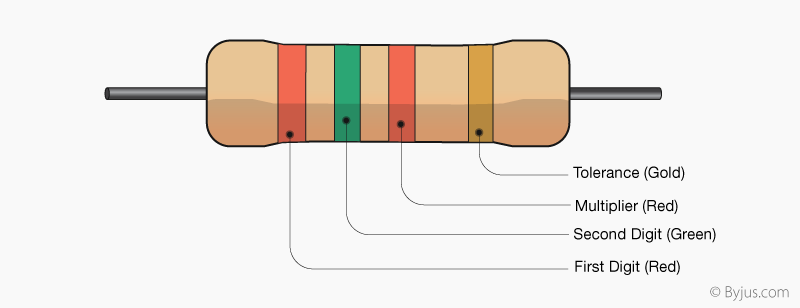
\includegraphics[width=3in]{../CMTolerance/Pics/resistor.png}
    \caption{\label{ResistorLabel}{\it Resistor labelling. Adapted
            from \url{https://byjus.com/physics/resistor-colour-codes/}.}}
\end{figure}
%
\begin{figure}[h]
    \center
    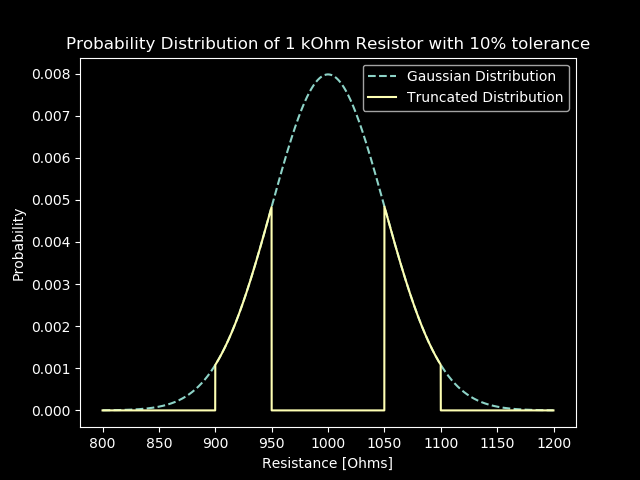
\includegraphics[width=3in]{../CMTolerance/Pics/tgauss_pdf_better.png}
    \caption{\label{trunc_guass}{\it Probability distribution for the
            value of a $10 k\Omega$ resistor with $\pm 10\%$ tolerance.
            Note the ``truncated Gaussian'' distribution.}}
\end{figure}
%
\begin{figure}[h]
    \center
    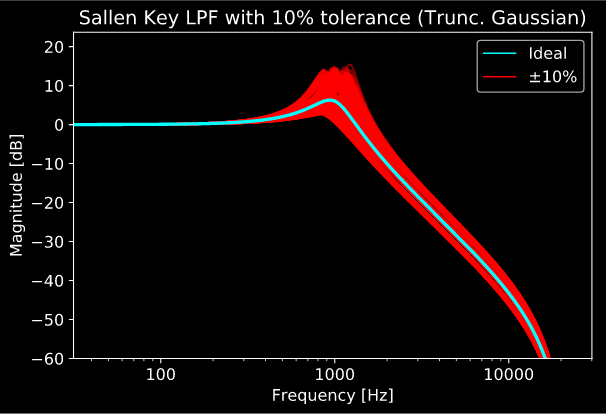
\includegraphics[width=3in]{../CMTolerance/Pics/lpf_tgauss_plot.png}
    \caption{\label{tol_LPF}{\it Frequency response of Sallen-Key lowpass
            filters made with components with $\pm 10\%$ tolerance.}}
\end{figure}
%
All resistors and capacitors are labelled with both a
component value (e.g. $1 k\Omega$ resistor, $1 \mu F$
capacitor), and a tolerance rating (e.g. $\pm 5\%$), as
shown in \cref{ResistorLabel}. We propose adjusting the
component values used in a circuit model to a random
value within the tolerance range of the component.
\newline\newline
When a manufacturer makes a batch of resistors or capacitors
the component values of the batch follows a roughly Gaussian
distribution centered at the ideal component value. The manufacturer
then extracts the worst components that can still satisfy a certain
tolerance rating and sells them at that rating \cite{tolerance}.
For example, if a
manufacturer sells resistors at $\pm 5\%$ and $\pm 10\%$ tolerance
the $\pm 10\%$ components will be distributed in a sort of ``truncated
Gaussian'' distribution, comprised of the original Gaussian
distribution truncated between 5 and 10\% (see \cref{trunc_guass}).
To show how component tolerances can affect the behavior of an audio
effect circuit, \cref{tol_LPF} shows the frequency responses of 1000
Sallen-Key lowpass filters made with components that have $\pm 10\%$
tolerance ratings.
%
%
\begin{figure}[h]
    \center
    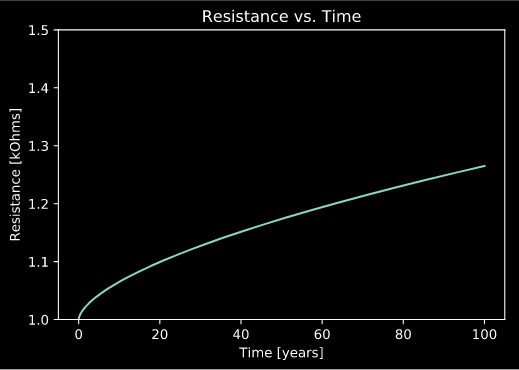
\includegraphics[width=3in]{../CMAging/Pics/r_time.png}
    \caption{\label{res-age}{\it $1 k\Omega$ Resistor aging over time.}}
\end{figure}
%
\section{Component Aging} \label{sec:age}
%
Another non-ideal factor that can affect the behavior of a circuit is
the aging of the components. This factor can be especially important
when examining vintage audio circuits.
%
\subsection{Resistor Aging} \label{sec:res-age}
%
As a resistor grows old, its resistance tends to increase. For a typical
thin-film resistor, the age dependence is described by the following
equation \cite{thermal_resistors}.
%
\begin{equation}
    \frac{\Delta R}{R} = (1.51 \times 10^{12})\ 
    t^{0.61}\  e^{- 15,087 / T}    
    \label{eq:resistor-age}
\end{equation}
%
where $t$ is the length of time the resistor has been used (in hours), and
$T$ is the operating temperature in Kelvins. In \cref{res-age}, we show
a $1 k\Omega$ resistor operating at 400 K running over a period of 100
years. While the resistance change may seem small, these small changes
compound over all the resistors in the circuit. \Cref{res-age-freq} shows
the frequency response of a Sallen-Key lowpass filter with resistor aging,
again with an operating temperature of 400 K.
%
\begin{figure}[h]
    \center
    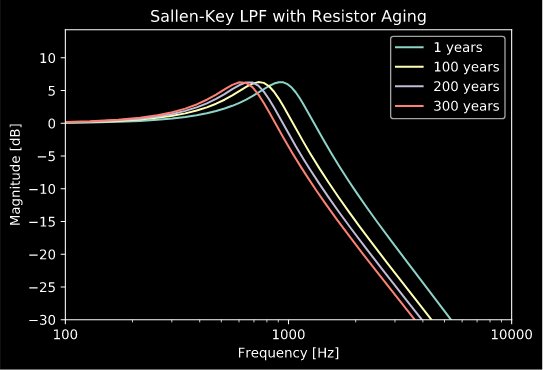
\includegraphics[width=3in]{../CMAging/Pics/r_freq.png}
    \caption{\label{res-age-freq}{\it Sallen-Key LPF with resistor aging.}}
\end{figure}
%
\begin{figure}[h]
    \center
    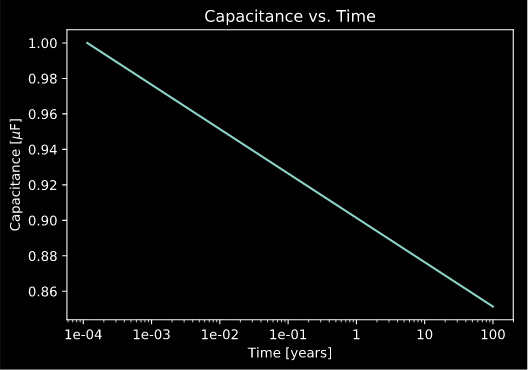
\includegraphics[width=3in]{../CMAging/Pics/cap_time.png}
    \caption{\label{cap-age}{\it Capacitor aging over time.}}
\end{figure}
%
\begin{figure}[h]
    \center
    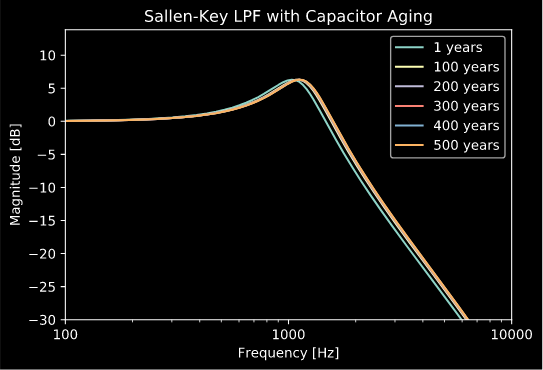
\includegraphics[width=3in]{../CMAging/Pics/cap_freq.png}
    \caption{\label{cap-age-freq}{\it Sallen-Key LPF with capacitor aging.}}
\end{figure}
%
\subsection{Capacitor Aging} \label{sec:cap-age}
%
For audio circuits, it is typical to use class II X7R capacitors, due to
their minimal amount of voltage dependence, meaning the resulting circuit
will have a minimal Total Harmonic Distortion (THD). For this class of
capacitor, the capacitance decreases by $\sim2.5\%$ per decade hour
\cite{cap-aging}. \Cref{cap-age} shows the capacitance of a $1 \mu F$
capacitor aging over a period of 100 years, and \cref{cap-age-freq} shows
the frequency response of a Sallen-Key lowpass filter with capacitor
aging.
%
\subsubsection{Capacitor Failure} \label{sec:cap-fail}
%
Capacitor aging again makes a minor difference to the overall behavior
of a circuit, however older circuit tend to have a larger issue with
capacitor failure. For the class of capacitor considered here, the
expected lifetime is approximately:
%
\begin{equation}
    L = (5000 \text{ hours})\ 2^{(373 - T) / 10}
    \label{eq:cap-fail}
\end{equation}
%
While there is some fluctuation in actual failure times, capacitor
lifetime tends to follow a normal distribution \cite{cap-fail}. When
a capacitor fails, its capacitance tends to increase to at least an
order of magnitude above its ideal value, and tends to have a large
dependence on the voltage across its terminals, resulting in a much
greater amount of THD.
%
\begin{figure}[h]
    \center
    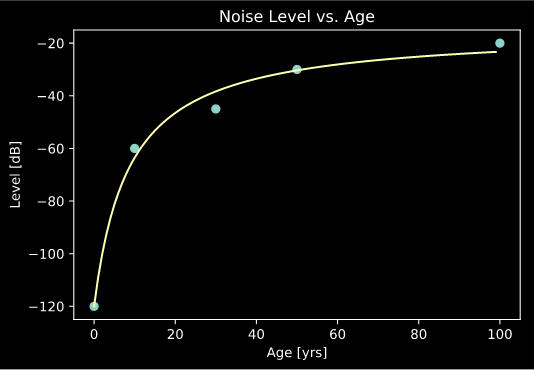
\includegraphics[width=3in]{../OpAmp/Pics/age_noise.png}
    \caption{\label{opamp-age-noise}{\it Op-amp noise over time.}}
\end{figure}
%
\begin{figure}[h]
    \center
    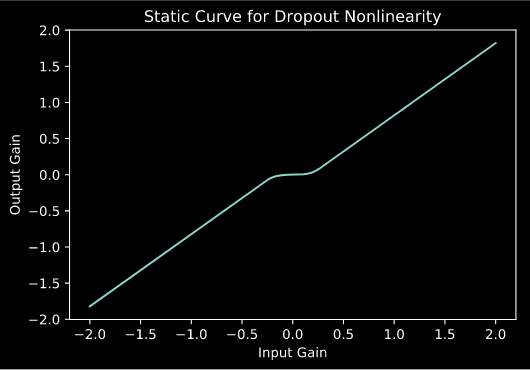
\includegraphics[width=3in]{Pics/dropout.png}
    \caption{\label{dropout}{\it Dropout nonlinearity.}}
\end{figure}
%
\subsection{Op-Amp Aging} \label{sec:opamp-age}
%
As op-amps age, they are subjected to shorts, and large currents across
their terminals, which causes them to develop a noise characteristic,
and lose some of their bandwidth \cite{opamp-age}. The noise power
increases with age, as shown in \cref{opamp-age-noise}.
\newline\newline
From our own measurements, we have found that as an op-amp ages and
approaches failure, it starts to exhibit a distortion characteristic
similar to the canonical ``dropout'' or ``dead-zone'' static nonlinearity,
shown in \cref{dropout}.
%
\begin{figure}[h]
    \center
    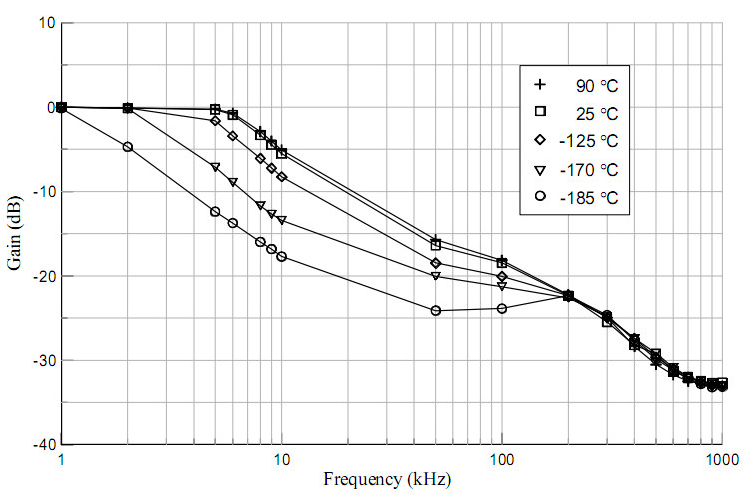
\includegraphics[width=3in]{Pics/NASA.png}
    \caption{\label{NASA}{\it Op-amp gain vs. frequency at various
        temperatures. Adapted from \cite{opamp-temp}.}}
\end{figure}
%
\begin{figure}[h]
    \center
    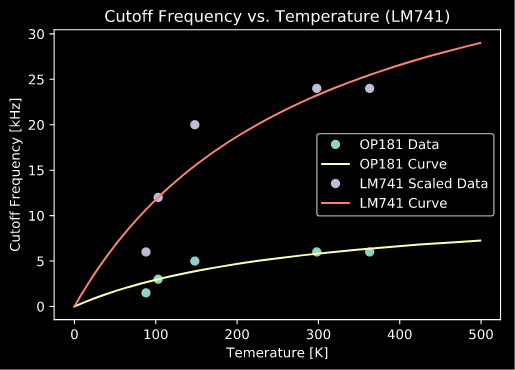
\includegraphics[width=3in]{../OpAmp/Pics/freq_temp_shift.png}
    \caption{\label{opamp-temp}{\it Cutoff frequency vs. temperature for
        OP181 and LM741 op-amps, including scaled data.}}
\end{figure}
%
\begin{figure}[h]
    \center
    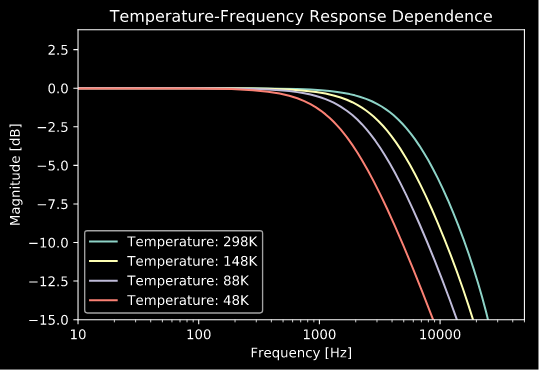
\includegraphics[width=3in]{../OpAmp/Pics/temp_freq_response.png}
    \caption{\label{opamp-temp-freq}{\it Frequency response of a Sallen-Key
        LPF with various op-amp temperatures.}}
\end{figure}
%
\section{Op-Amp Temperature} \label{sec:temp}
%
The operating temperature at which a circuit is used can also have an
affect on the circuit's overall sound. In particular, op-amps tend to
have a relatively strong temperature dependence, particularly in relation
to the op-amp's bandwidth. \cite{opamp-temp} describes a NASA study
examining the temperature dependent behavior of the Analog Devices OP181
op-amp, though their results can be scaled to apply to most other op-amp's
with similar construction. \Cref{NASA} shows the frequency response of the
OP181 at various temperatures.
\newline\newline
We propose scaling the data from \cite{opamp-temp} to apply to the widely
used Texas Instruments LM741 op-amp, and model the frequency response
using a first-order lowpass filter, with cutoff frequency $f_c$ dependent
on the operating temperature. We determined that the relationship between
temperature and $f_c$ follows the form of a ``binding'' function, as follows:
%
\begin{equation}
    f_c(T) = \frac{30.96 T}{T + 290.48}  
    \label{eq:binding}
\end{equation}
%
where $T$ is the operating temperature in Kelvin. \Cref{opamp-temp} shows
the data from the OP181 (adapted from \cite{opamp-temp}) and the scaled
data from the LM741, as well as the binding functions that best fit the
data. In \cref{opamp-temp-freq}, we show the frequency response of a
Sallen-Key lowpass filter with an LM741 op-amp at various operating
temperatures.
%
\begin{figure}[h]
    \center
    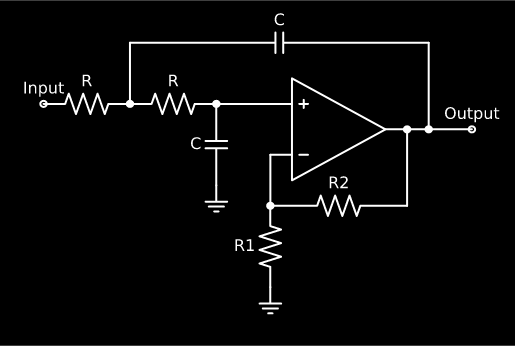
\includegraphics[width=3in]{../CMTolerance/Pics/sallen-key.png}
    \caption{\label{sallenkey}{\it Sallen-Key LPF circuit.}}
\end{figure}
%
\section{Implementation} \label{sec:impl}
%
\subsection{Sallen-Key Lowpass Filter} \label{sec:SK-LPF}
%
In the process of this study, we have been using a Sallen-Key lowpass
filter \cite{SallenKey} (see \cref{sallenkey}) as an example circuit for
examining the effects of the non-ideal factors described in the above
sections. The Sallen-Key LPF circuit is useful for testing, because it
lends itself easily to simple nodal analysis, assuming that the op-amp
in the circuit provides strictly linear gain (there is already existing
literature that examines models of the circuit where this assumption is
relaxed, e.g. \cite{SKF-DAFX}). Specifically, the transfer function of
this circuit can be written as
%
\begin{equation}
    H(s) = \frac{1}{\left(\frac{s}{2\pi f_c} \right)^2
         + \frac{1}{Q}\left(\frac{s}{2\pi f_c} \right) + 1}  
    \label{eq:SKF-transfer}
\end{equation}
%
where
%
\begin{equation}
    f_c = \frac{1}{2\pi RC}, \;\;
    Q = \frac{1}{2 - \frac{R_2}{R_1}}
    \label{eq:SKF-params}
\end{equation}
%
\Cref{tol_LPF,res-age-freq,cap-age-freq,opamp-temp-freq} show the
frequency responses of the Sallen-Key lowpass filter circuit for
each of the non-ideal factors discussed above.

\subsection{WDF Diode Clipper} \label{sec:WDF}
%
\begin{figure}[h]
    \center
    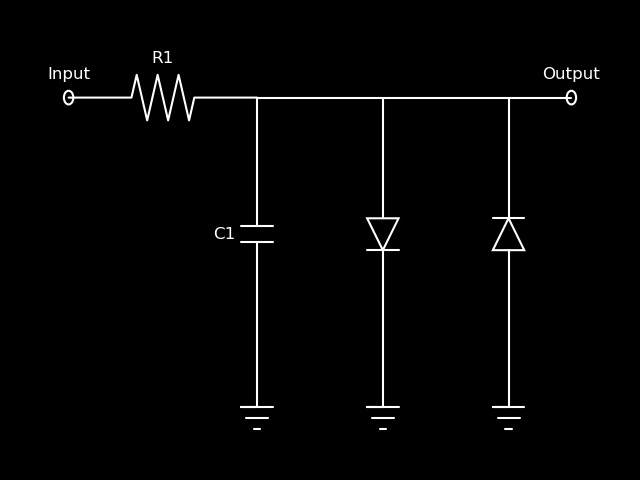
\includegraphics[width=3in]{Pics/diodeclipper.png}
    \caption{\label{diodeclipper}{\it Diode clipper circuit.}}
\end{figure}
%
As a second example circuit, we chose to implement a diode clipper using
the Wave Digital Filter (WDF) formulation. Originally, developed by
Alfred Fettweis \cite{Fettweis} in the 1980's, and expanded on in recent
years by Yeh \cite{YehWDF}, Werner \cite{KurtThesis}, and others
\cite{JJWDF,WDF2}, WDFs provide a particularly well suited circuit
modelling method for incorporating non-ideal factors, due to their highly
modular nature. We implemented a wave digital emulation of a simple diode
clipper circuit (see \cref{diodeclipper}), based on the formulations
derived in \cite{YehDiode,KurtDiode}, including all non-ideal factors
described above.

\subsection{Software Implementation} \label{sec:soft-impl}
%
The Sallen-Key lowpass filter and diode clipper models have been implemented
as audio plugins (VST/AU) using the JUCE/C++ framework. In each plugin,
the user can control various parameters related to the component
tolerances, age, and temperature, to see how these factors effect the
overall sound of the circuit model. The plugins and their source code are
freely available on GitHub
\footnote{\url{https://github.com/jatinchowdhury18/Bad-Circuit-Modelling}}.

\section{Conclusion} \label{sec:conclusion}
%
In this paper we have discussed non-ideal circuit factors, including
component tolerance, age, and temperature, and shown how these factors
can be implemented into existing circuits modelled with nodal analysis
and wave digital techniques.
\newline\newline
The main limitation in this line of research has been the lack of
reliable and rigorous sources discussing non-ideal circuit factors.
Each of the factors discussed here have been verified experimentally
by the author to the greatest possible extent, however future research
could include more rigorous testing of component tolerance distributions,
age dependence, and more. Another future line of research involves the
possibility of including random factors in consumer audio software, perhaps
by seeding a random number generator based on the time at which the
software is installed, so that each user has a copy of the software that
sounds slightly unique.

\section{Acknowledgments}
%
The author would like to thank Andrew Garver for inspiration, Jingjie Zhang
and Kurt Werner for providing sound and patient advice regarding WDFs, and the
GASP working group for their gratious support and vital feedback.

%\newpage
% \nocite{*}
\bibliographystyle{IEEEbib}
\bibliography{references}

\end{document}
